\documentclass[11pt]{article}

\usepackage{amsmath}
\usepackage[margin=1.0in]{geometry}
\usepackage[utf8]{inputenc}
\usepackage[T1]{fontenc}

\title{Generating economic scenarios in \texttt{StocVal}}
\author{Nathan Esau}
\date{}

\usepackage{Sweave}
\begin{document}
\Sconcordance{concordance:var_canada_summary.tex:var_canada_summary.Rnw:%
1 11 1 1 0 9 1 1 3 2 0 1 1 1 2 1 0 1 1 4 0 2 2 1 0 1 2 5 0 2 2 1 0 1 2 %
5 0 1 2 21 1 1 6 5 0 1 6 5 0 1 1 11 0 1 2 1 1 1 2 1 0 1 5 4 0 1 2 1 0 1 %
1 1 6 5 0 1 1 3 0 1 2 1 1 1 2 129 0 1 2 4 1 1 2 1 0 4 1 1 5 7 0 1 2 4 1 %
1 3 2 0 1 2 1 0 1 1 4 0 1 2 1 3 2 0 1 2 1 0 1 1 4 0 1 2 1 3 2 0 1 2 1 0 %
1 1 4 0 1 2 1 3 2 0 1 2 1 0 1 1 4 0 1 2 1 3 2 0 1 2 1 0 1 1 4 0 1 2 1 1}


\maketitle

\section{Historical data}

\subsection{Time series plots}

The data used is plotted below. The reference period is 199501:201505.
\begin{Schunk}
\begin{Sinput}
> market_data <- 
+     readRDS("~/Dropbox/Research/StocVal/data/Canada/varinput_canada.Rda")
> yield_dataTS <- ts(market_data[,2:8],start = 1995, end=2015, freq=12)
> plot(yield_dataTS, col=1:7, plot.type="single", ylab="Yield", 
+     main="Historical continuously compounded monthly yields")
> legend("topright", legend=colnames(yield_dataTS), ncol=2, lty=1, col=1:8)
\end{Sinput}
\end{Schunk}
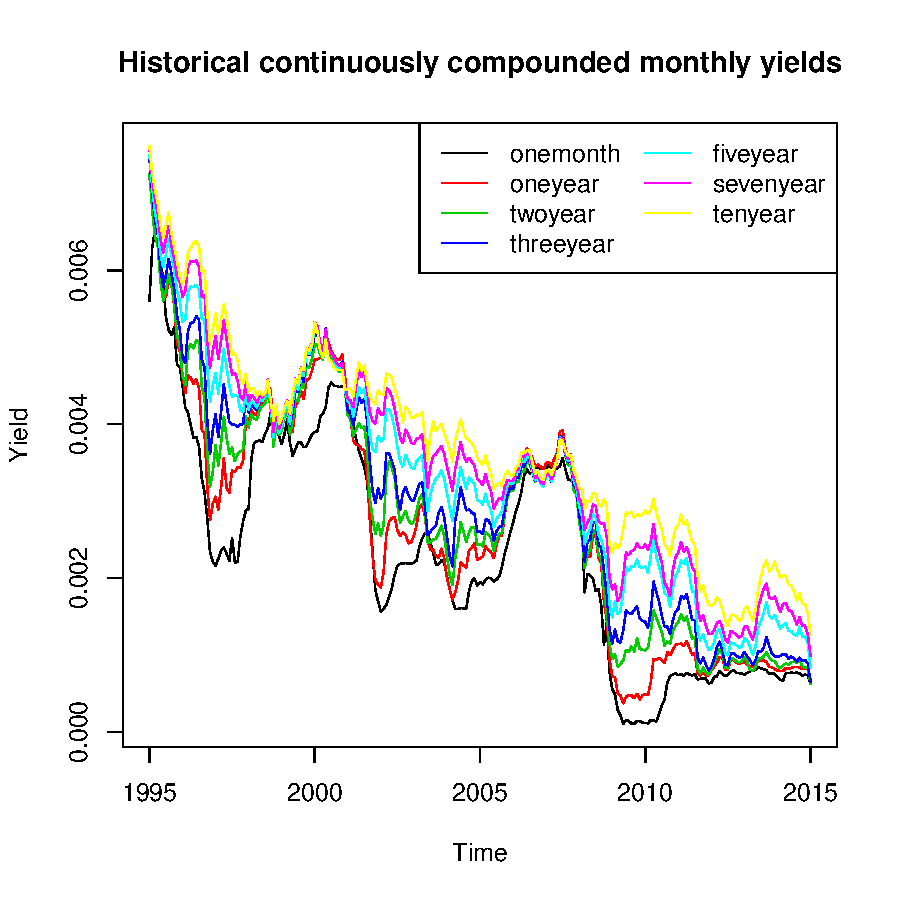
\includegraphics{var_canada_summary-001}

\begin{Schunk}
\begin{Sinput}
> stock_TS <- ts(market_data[,9], start=1995, end=2015, freq=12)
> plot(stock_TS, ylab="Stock return", main="Historical continuously compounded
+      monthly stock returns")
\end{Sinput}
\end{Schunk}
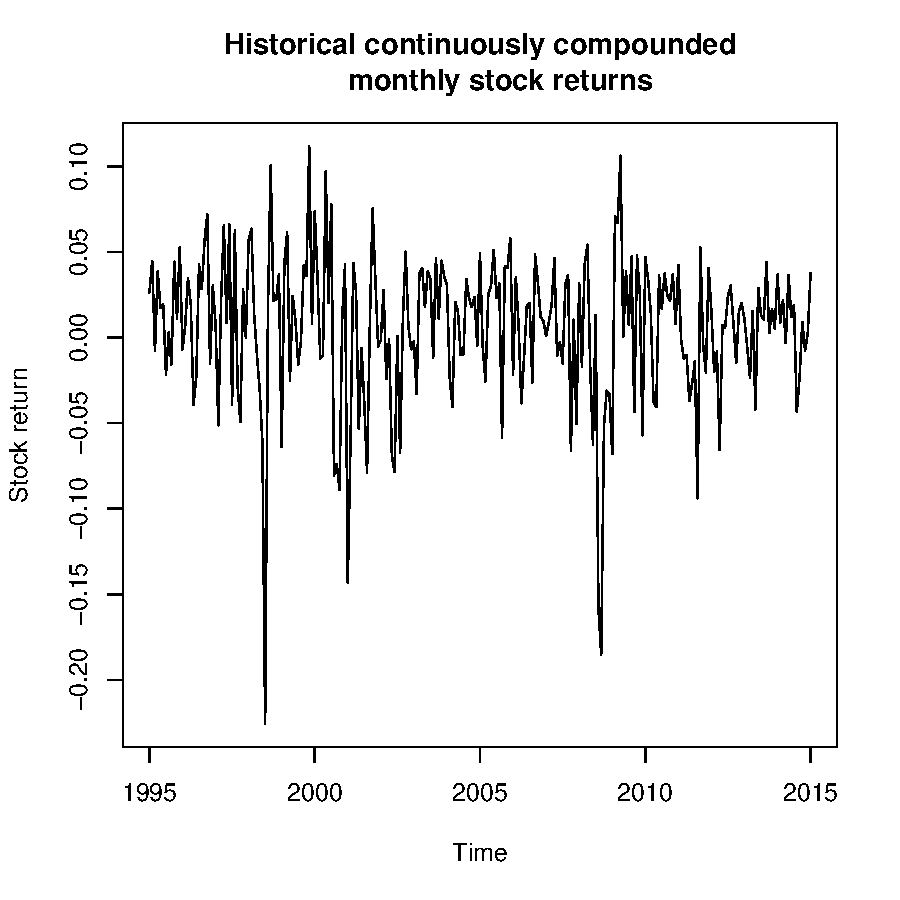
\includegraphics{var_canada_summary-002}

\begin{Schunk}
\begin{Sinput}
> inflation_TS <- ts(market_data[,10], start=1995, end=2015, freq=12)
> plot(inflation_TS, ylab="Inflation", main="Historical continuously compounded
+      monthly inflation rates")
\end{Sinput}
\end{Schunk}
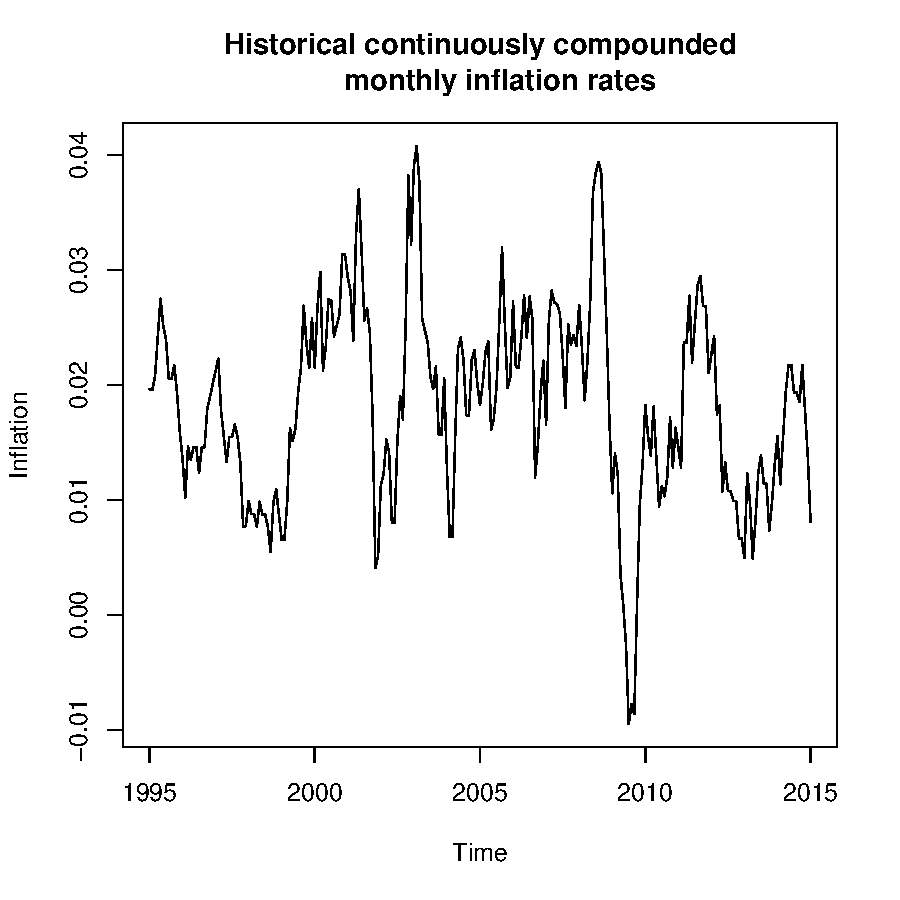
\includegraphics{var_canada_summary-003}

\section{VAR in \texttt{StocVal}}

\subsection{Model}
To generate economic scenarios, a five component VAR model was used. 

\begin{align*}
X_t - \mu &= \Phi (X_{t-1} - \mu) + \Sigma \epsilon_{t} \\
X_t &= \left( 
\begin{matrix}
    y_t^{(1)} \\ 
    \pi_t \\ 
	y_t^{(120)} \\ 	
	x_t \\ 
	y_t^{(12)}
\end{matrix} 
\right)
\end{align*}

where $y_t^{(n)}$ is the $n-month$ continuously compounded monthly zero coupon yield rate, $\pi_y$ is the continuously compounded monthly inflation rate and $x_t$ is the continuously compounded monthly return on a stock index. $\mu$ is a 5x1 vector containing the historical means.

First, the historical means are shown.
\begin{Schunk}
\begin{Sinput}
> var_data <- data.frame(onemonth=market_data$onemonth,
+    inflation=market_data$inflation, 
+    tenyear=market_data$tenyear,
+    stock=market_data$stock,
+    oneyear=market_data$oneyear)
> mu <- matrix(c(mean(var_data$onemonth),
+    mean(var_data$inflation),
+    mean(var_data$tenyear),
+    mean(var_data$stock),
+    mean(var_data$oneyear)),
+    5, 1)
> print(mu)
\end{Sinput}
\begin{Soutput}
            [,1]
[1,] 0.002305719
[2,] 0.018206346
[3,] 0.003660959
[4,] 0.005253706
[5,] 0.002648492
\end{Soutput}
\end{Schunk}

Next, the VAR parameters are calculated using the \texttt{vars} package.
\begin{Schunk}
\begin{Sinput}
> library(vars)
> var_input <- data.frame(onemonth=var_data$onemonth - mu[1], 
+    inflation=var_data$inflation - mu[2],
+    tenyear=var_data$tenyear - mu[3],
+    stock=var_data$stock - mu[4],
+    oneyear=var_data$oneyear - mu[5])
> # fit var(1)
> var_model <- VAR(var_input, p=1, type = "none")
> Phi <- coef(var_model)
> Phi <- matrix( c(Phi$onemonth[,1],
+    Phi$inflation[,1],
+    Phi$tenyear[,1],
+    Phi$stock[,1],
+    Phi$oneyear[,1]),
+    5, 5, byrow=TRUE)
> Sigma <- summary(var_model)$covres 
\end{Sinput}
\end{Schunk}

\subsection{Estimation results}
\begin{Schunk}
\begin{Sinput}
> print(summary(var_model))
\end{Sinput}
\begin{Soutput}
VAR Estimation Results:
========================= 
Endogenous variables: onemonth, inflation, tenyear, stock, oneyear 
Deterministic variables: none 
Sample size: 244 
Log Likelihood: 6953.256 
Roots of the characteristic polynomial:
0.9772 0.8982 0.8784 0.8784 0.1639
Call:
VAR(y = var_input, p = 1, type = "none")


Estimation results for equation onemonth: 
========================================= 
onemonth = onemonth.l1 + inflation.l1 + tenyear.l1 + stock.l1 + oneyear.l1 

               Estimate Std. Error t value Pr(>|t|)    
onemonth.l1   0.6239391  0.0345784  18.044  < 2e-16 ***
inflation.l1 -0.0015483  0.0011317  -1.368    0.173    
tenyear.l1   -0.0979380  0.0148007  -6.617 2.38e-10 ***
stock.l1      0.0001353  0.0002058   0.657    0.511    
oneyear.l1    0.4263204  0.0385021  11.073  < 2e-16 ***
---
Signif. codes:  0 ‘***’ 0.001 ‘**’ 0.01 ‘*’ 0.05 ‘.’ 0.1 ‘ ’ 1


Residual standard error: 0.0001388 on 239 degrees of freedom
Multiple R-Squared: 0.9915,	Adjusted R-squared: 0.9913 
F-statistic:  5565 on 5 and 239 DF,  p-value: < 2.2e-16 


Estimation results for equation inflation: 
========================================== 
inflation = onemonth.l1 + inflation.l1 + tenyear.l1 + stock.l1 + oneyear.l1 

              Estimate Std. Error t value Pr(>|t|)    
onemonth.l1  -0.303257   1.024771  -0.296    0.768    
inflation.l1  0.867000   0.033539  25.851   <2e-16 ***
tenyear.l1   -0.309748   0.438636  -0.706    0.481    
stock.l1      0.005081   0.006099   0.833    0.406    
oneyear.l1    0.801839   1.141053   0.703    0.483    
---
Signif. codes:  0 ‘***’ 0.001 ‘**’ 0.01 ‘*’ 0.05 ‘.’ 0.1 ‘ ’ 1


Residual standard error: 0.004114 on 239 degrees of freedom
Multiple R-Squared: 0.7744,	Adjusted R-squared: 0.7697 
F-statistic: 164.1 on 5 and 239 DF,  p-value: < 2.2e-16 


Estimation results for equation tenyear: 
======================================== 
tenyear = onemonth.l1 + inflation.l1 + tenyear.l1 + stock.l1 + oneyear.l1 

               Estimate Std. Error t value Pr(>|t|)    
onemonth.l1   0.0885309  0.0377403   2.346   0.0198 *  
inflation.l1 -0.0019696  0.0012352  -1.595   0.1121    
tenyear.l1    0.9879540  0.0161541  61.158   <2e-16 ***
stock.l1     -0.0001899  0.0002246  -0.845   0.3988    
oneyear.l1   -0.0825834  0.0420228  -1.965   0.0505 .  
---
Signif. codes:  0 ‘***’ 0.001 ‘**’ 0.01 ‘*’ 0.05 ‘.’ 0.1 ‘ ’ 1


Residual standard error: 0.0001515 on 239 degrees of freedom
Multiple R-Squared: 0.9879,	Adjusted R-squared: 0.9877 
F-statistic:  3906 on 5 and 239 DF,  p-value: < 2.2e-16 


Estimation results for equation stock: 
====================================== 
stock = onemonth.l1 + inflation.l1 + tenyear.l1 + stock.l1 + oneyear.l1 

             Estimate Std. Error t value Pr(>|t|)  
onemonth.l1   1.75991   10.79950   0.163   0.8707  
inflation.l1 -0.73605    0.35345  -2.082   0.0384 *
tenyear.l1    3.61771    4.62254   0.783   0.4346  
stock.l1      0.15841    0.06428   2.465   0.0144 *
oneyear.l1   -2.86903   12.02494  -0.239   0.8116  
---
Signif. codes:  0 ‘***’ 0.001 ‘**’ 0.01 ‘*’ 0.05 ‘.’ 0.1 ‘ ’ 1


Residual standard error: 0.04335 on 239 degrees of freedom
Multiple R-Squared: 0.05844,	Adjusted R-squared: 0.03874 
F-statistic: 2.967 on 5 and 239 DF,  p-value: 0.01283 


Estimation results for equation oneyear: 
======================================== 
oneyear = onemonth.l1 + inflation.l1 + tenyear.l1 + stock.l1 + oneyear.l1 

               Estimate Std. Error t value Pr(>|t|)    
onemonth.l1  -0.1583894  0.0441307  -3.589 0.000403 ***
inflation.l1 -0.0014850  0.0014443  -1.028 0.304905    
tenyear.l1   -0.0361308  0.0188894  -1.913 0.056975 .  
stock.l1     -0.0001443  0.0002627  -0.549 0.583335    
oneyear.l1    1.1579686  0.0491383  23.566  < 2e-16 ***
---
Signif. codes:  0 ‘***’ 0.001 ‘**’ 0.01 ‘*’ 0.05 ‘.’ 0.1 ‘ ’ 1


Residual standard error: 0.0001772 on 239 degrees of freedom
Multiple R-Squared: 0.9873,	Adjusted R-squared: 0.987 
F-statistic:  3705 on 5 and 239 DF,  p-value: < 2.2e-16 



Covariance matrix of residuals:
           onemonth  inflation   tenyear      stock   oneyear
onemonth  1.883e-08  6.387e-08 5.604e-09  3.120e-07 1.431e-08
inflation 6.387e-08  1.692e-05 4.698e-08 -1.793e-05 7.258e-08
tenyear   5.604e-09  4.698e-08 2.231e-08  3.538e-07 1.784e-08
stock     3.120e-07 -1.793e-05 3.538e-07  1.879e-03 4.236e-07
oneyear   1.431e-08  7.258e-08 1.784e-08  4.236e-07 3.064e-08

Correlation matrix of residuals:
          onemonth inflation tenyear    stock oneyear
onemonth   1.00000   0.11316 0.27343  0.05245 0.59601
inflation  0.11316   1.00000 0.07646 -0.10057 0.10080
tenyear    0.27343   0.07646 1.00000  0.05463 0.68211
stock      0.05245  -0.10057 0.05463  1.00000 0.05582
oneyear    0.59601   0.10080 0.68211  0.05582 1.00000
\end{Soutput}
\end{Schunk}

\subsection{Example scenario}
Next we generate a VAR scenario for the next 25 year (300 months) and plot
the resulting time series. To generate random numbers from a multivariate standom
normal distribution, the \texttt{MASS} package is used.
\begin{Schunk}
\begin{Sinput}
> library(MASS)
> Xt <- matrix(as.numeric(tail(var_input, 1)), 5, 1)
> path <- matrix(0, 5, 301)
> path[,1] <- Xt
> set.seed(137531)
> for(i in 1:300) {
+     rand <- mvrnorm(n=1, mu=rep(0,5), Sigma=Sigma)
+     Xt <- Phi %*% Xt + rand
+     path[,i+1] <- Xt 
+ }
\end{Sinput}
\end{Schunk}

The path of each of the variables is shown below (the projected values are the ones 
to the right of the dotted line).

\subsection{Projection plots}
\begin{Schunk}
\begin{Sinput}
> onemonth_TS_combined <- ts(c(var_input$onemonth, path[1,]),
+     start=1995, end=2040, freq=12)
> plot(onemonth_TS_combined, ylab="One month yield rate", main="Continuously
+     compounded monthly one-month yield rate")
> abline(v=c(2015,6),lty=2)
\end{Sinput}
\end{Schunk}
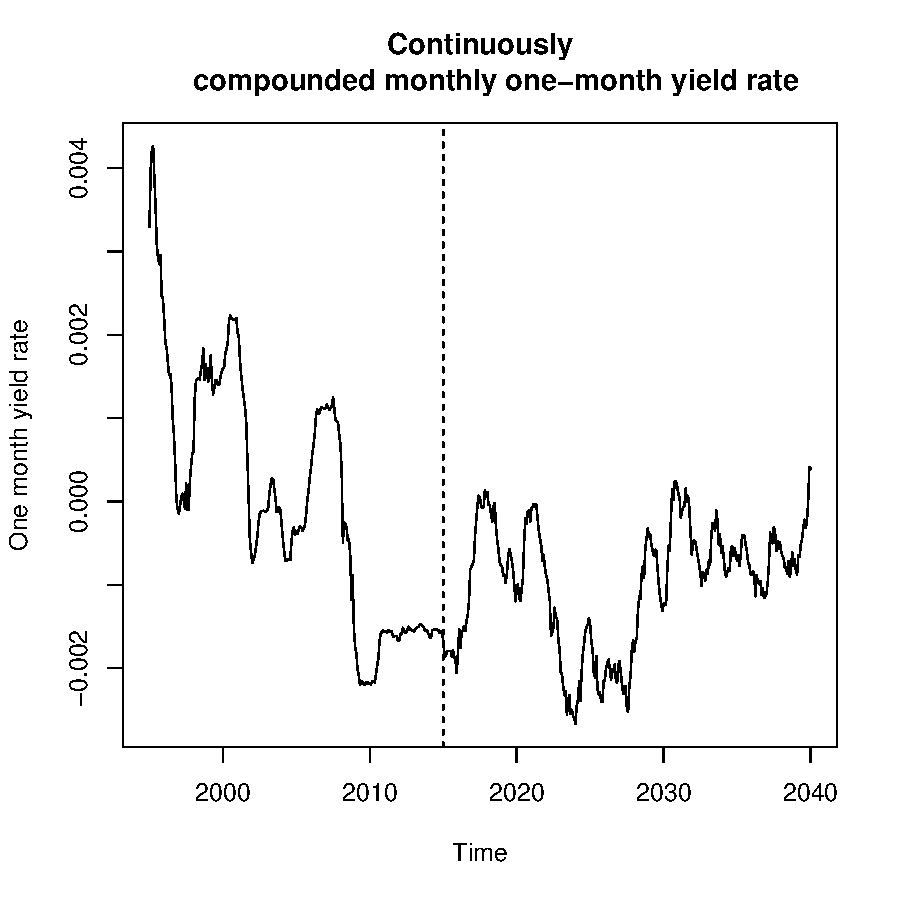
\includegraphics{var_canada_summary-008}

\begin{Schunk}
\begin{Sinput}
> inflation_TS_combined <- ts(c(var_input$inflation, path[2,]),
+     start=1995, end=2040, freq=12)
> plot(inflation_TS_combined, ylab="Inflation", main="Continuously compounded
+      monthly inflation rates", type='l')
> abline(v=c(2015,6), lty=2)
\end{Sinput}
\end{Schunk}
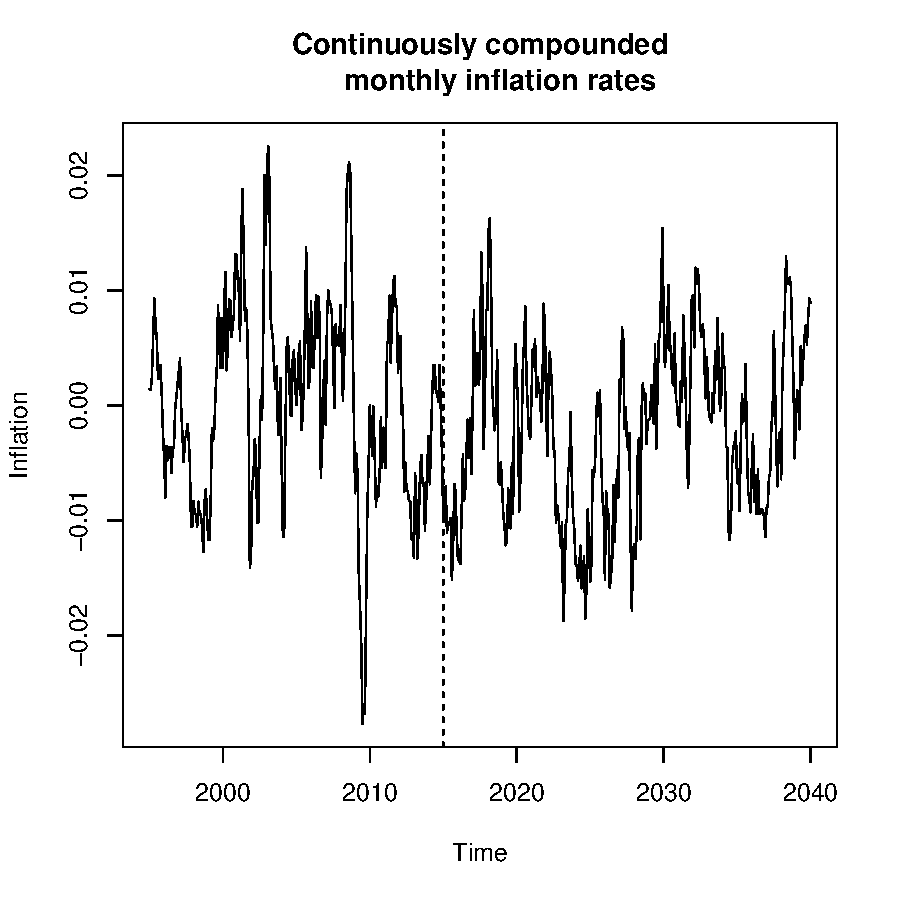
\includegraphics{var_canada_summary-009}

\begin{Schunk}
\begin{Sinput}
> tenyear_TS_combined <- ts(c(var_input$tenyear, path[3,]),
+     start=1995, end=2040, freq=12)
> plot(tenyear_TS_combined, ylab="Ten year yield rate", main="Continuously 
+     compounded monthly ten year yield rate")
> abline(v=c(2015,6), lty=2)
\end{Sinput}
\end{Schunk}
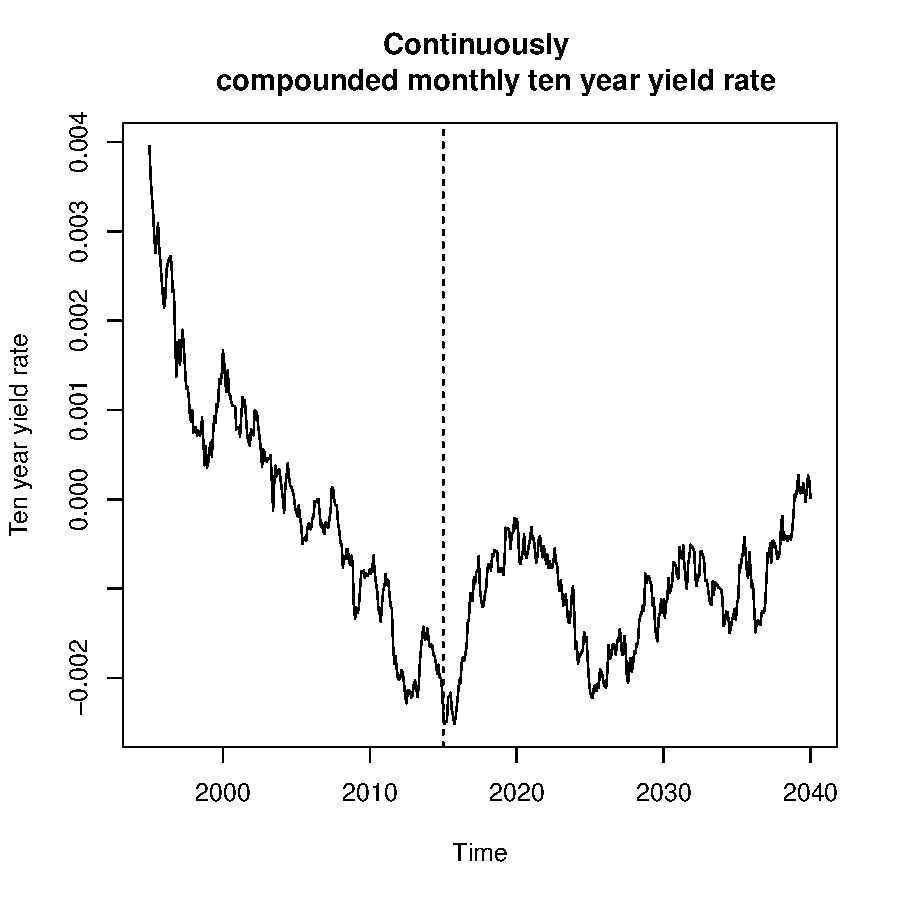
\includegraphics{var_canada_summary-010}

\begin{Schunk}
\begin{Sinput}
> stock_TS_combined <- ts(c(var_input$stock, path[4,]),
+     start=1995, end=2040, freq=12)
> plot(stock_TS_combined, ylab="Stock Price", main="Historical continuously compounded
+     stock returns", type='l')
> abline(v=c(2015,6), lty=2)
\end{Sinput}
\end{Schunk}
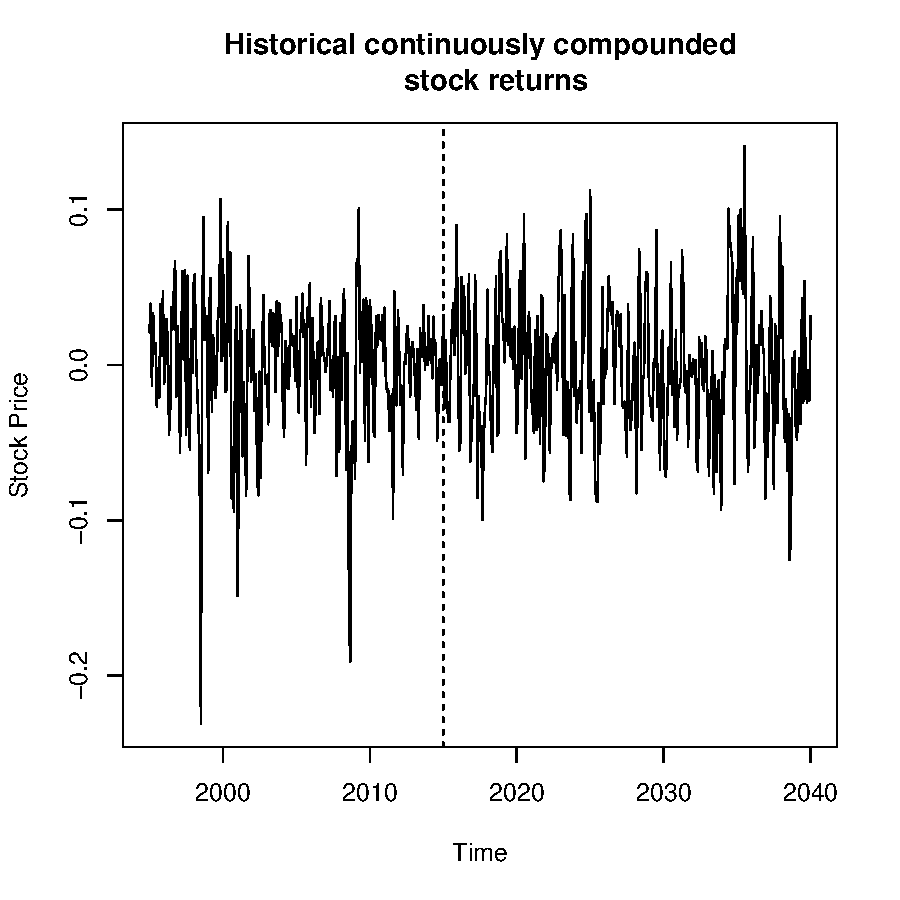
\includegraphics{var_canada_summary-011}

\begin{Schunk}
\begin{Sinput}
> oneyear_TS_combined <- ts(c(var_input$oneyear, path[5,]),
+     start=1995, end=2040, freq=12)
> plot(oneyear_TS_combined, ylab="One year yield rate", main="Continuously
+      compounded monthly one year yield rate")
> abline(v=c(2015,6), lty=2)
\end{Sinput}
\end{Schunk}
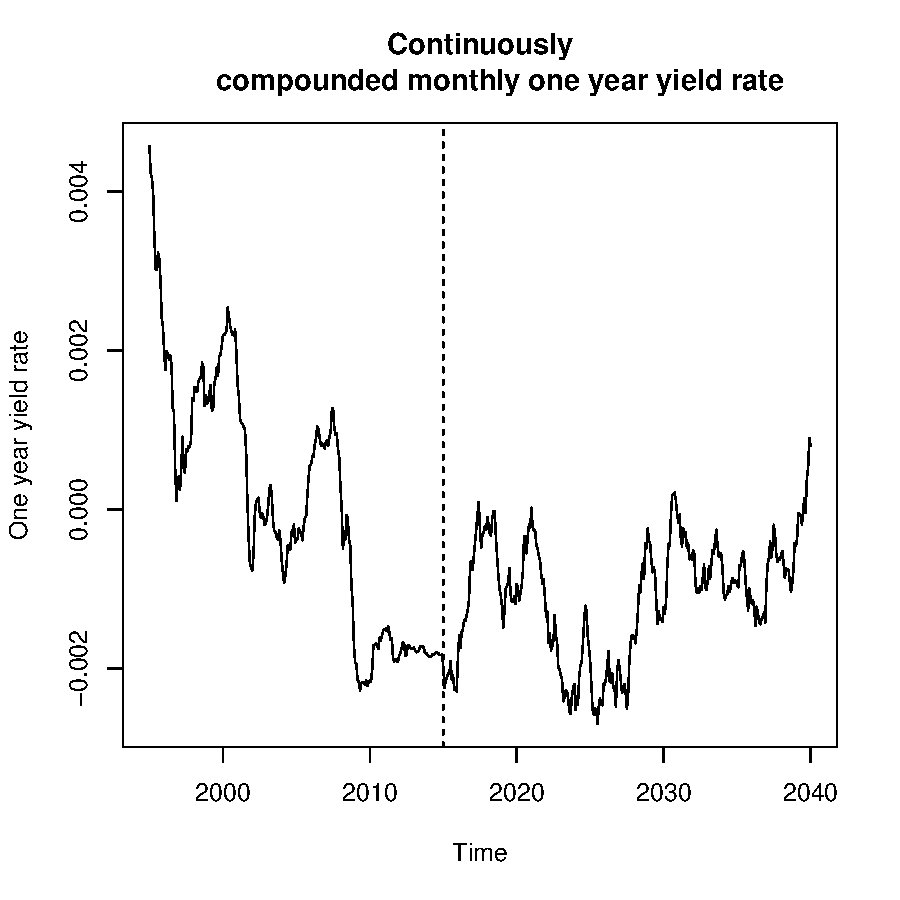
\includegraphics{var_canada_summary-012}

\end{document}
